\section{Work Plan and Execution Schedule}
\label{chp:workplan-schedule}

The work plan is to apply the two research methods as concurrently as possible while continuously developing the mentioned FLOSS tools. We divided the research work into four phases, each one producing a new iteration of the taxonomy describing the workflows of the Linux kernel development model.

\subsection{Phase I: Ethnographic Case Study I}

In the first phase, the doctoral student immersed himself not so profoundly into the Linux ecosystem by exploring the dynamics of contributing to some parts of the ecosystem and mentoring graduate and undergraduate students as newcomers. In a sense, we dip ourselves into the ecosystem while observing how the movement of new developers into it works.

\paragraph{P1.1: Exploration into the Linux ecosystem.}
The doctoral student re-acclimated himself with the Linux kernel ecosystem by sending simple and exploratory patches to the AMD GPU, IIO, and staging. He also recompiled the experiences of fellow researchers and members of the Linux community by reading their blog posts, some academic publications, and through direct conversations.

\paragraph{P1.2: Mentor newcomers I.}
In the first semester of 2024, the \textit{Free Software Development} course ministered at IME-USP dedicated the first three-fourths of the discipline program to mentoring around 30 graduated and undergraduate students that involved teaching them how to: set up a testing environment; configure, compile, install, and boot a custom Linux kernel from source code; develop changes; send changes as contributions and participate in the review process; and much more. Essentially, lead them through all the steps described in the concept map of Figure \ref{fig:patch-development-workflow}. To accomplish this, students did in-person workshops based on tutorials devised by past researchers from the Software Systems Research Group of IME-USP, who are veteran Linux developers. The doctoral student was the principal mentor in this process. At the end of the course, students filled out a survey to collect data about their experiences.

\paragraph{\underline{\textit{P1.3}}: kw/patch-hub dev I.}
kw has been in development since 2019, and it already encoded many solutions for workflows at the start of 2024. In this first phase, the doctoral student invested great effort and time in developing, maintaining, and bringing new contributors to the project. From February to August, the doctoral student was also a mentor in \textit{Google Summer of Code 2024} (GSoC 24) for two contributors in kw. The doctoral student transformed patch-hub - which was a proof-of-concept tool implemented in Bash script inside the kw codebase - into a dedicated project with its own codebase and written in Rust. During July, the doctoral student fully migrated the tool to the new project and surpassed its features, performance, and maintainability, which were unacceptable in the old form. Throughout the remainder of the second term of 2024, the project started to have recurring contributors forming a small community and really elevating it to a FLOSS project.

\subsection{Phase II: Ethnographic Case Study II}
The second phase continues the first phase, although the doctoral student deepens the immersion into the ecosystem by making more meaningful contributions and trying to be trusted with some maintainer responsibilities. Mentoring newcomers is virtually the same as in Phase I, but the researchers also conduct a first trial of experiments.\looseness=-1

\paragraph{P2.1: Deep immersion into the Linux ecosystem.}
The doctoral student submits contributions that have a more profound impact on Linux subprojects and also engages in reviews sent from other contributors. The idea is to experience the role of non-casual contributors and, at least, experience one of the major responsibilities of maintainers, which is reviewing proposed changes. Additionally, the doctoral student will try to undertake formal responsibilities as a maintainer by organically and politely escalating his importance in the subproject(s).

\paragraph{P2.2: Mentor newcomers II.}
With another offering of the Free Software Development course in the first semester of 2025, mentoring newcomers will take the same shape, apart from natural adaptations and changes that resulted from the lessons learned in the first mentoring.

\paragraph{P2.3: Conduct Experiments I (newcomers).}
In the middle of the workshop series of \textbf{P2.2}, half of the course students will be randomly selected to use kw tools from that point onwards, while the other half will maintain use of the same tools used in the first mentoring. The overall program will remain the same, diverging from the tools used. Data describing the impact of including the use of kw tools will be collected through a survey, which will enable us to derive qualitative metrics, like how well bottleneck \textit{X} of workflow \textit{Y} was mitigated by kw \textit{Z} tool(s), and also quantitative metrics like measure how much time workflow \textit{W} demanded with and without the use of kw.

\paragraph{\underline{\textit{P2.4}}: kw/patch-hub dev II.}
With a better understanding of core workflows, in the second phase, the development of kw will focus on maintaining and refining the existing features it has while making a patch-hub with features enough to be included in a developer routine. The doctoral student is, once again, mentoring a contributor in GSoC 25. However, the work is focused on patch-hub. 

\subsection{Phase III: Unbiased Perspectives}

Through ethnographic case studies, we can get valuable information from closely observing and immersing ourselves in the Linux development model. However, there are some innate biases regarding how the researchers (and their associates) view the ecosystem and the subset of the ecosystem considered. To mitigate this, triangulating these results with academic and grey literature, along with the perspective of the community and its key players, is necessary.

\paragraph{P3.1: Conduct Multivocal Literature Review.}
Here, the researchers will cross the state-of-the-art from the last 5 years about Linux kernel development, focusing on workflows, with state-of-the-practice from community publications like blog posts, articles, and mailing lists.

\paragraph{P3.2: Collect feedback from the Linux community and its key players at events.}
In previous research works done by past researchers from our research group, the board of the Linux Foundation requested that feedback from the community and key players be collected by participating in in-loco events and direct exchange instead of requesting surveys. Given this guidance, the researchers, especially the doctoral student, aim to participate in events such as \textit{FOSDEM}\footnote{\href{https://fosdem.org/2025/}{FOSDEM 2025 site.}}, as a speaker presenting the kw project and patch-hub, to interact with these sources of valuable information (which the student did on this DebConf 2025\footnote{\href{https://debconf25.debconf.org/schedule/}{DebConf 2025 schedule.}})

\paragraph{\underline{\textit{P3.3}}: kw/patch-hub dev III.} Leveraging \textbf{Taxonomy I}, incorporate its knowledge in developing kw and patch-hub.

\subsection{Phase IV: Final Validation.}
From the coalition of the results from Phase I and II with Phase III, we aim to validate our reviewed theoretical framework describing the Linux kernel development model in a real-world scenario through experiments with veteran Linux developers.

\paragraph{P4.1: Conduct Experiments II (real practitioners).}
To capture the actual workflows of practitioners, this trial of experiments will be conducted by having veteran developers follow their day-to-day tasks naturally while using kw tools and patch-hub. Data will be generated seamlessly using kw, which already keeps statistics of some actions locally, like how many times the user compiled the kernel and the minimum, maximum, and average time it took for each day or period. Data telemetry is being investigated and planned to be implemented in the project soon. It will be inspired in the \textit{Debian Popularity Contest}, where Debian users that comply send data about Debian packages to servers and go through a data anonymization process before analysis.

\paragraph{\underline{\textit{P4.2}}: kw/patch-hub dev IV.} Leveraging \textbf{Taxonomy II}, incorporate its knowledge in developing kw and patch-hub.

\subsection{Work Plan Overview}

\begin{figure}[ht]
    \centering
    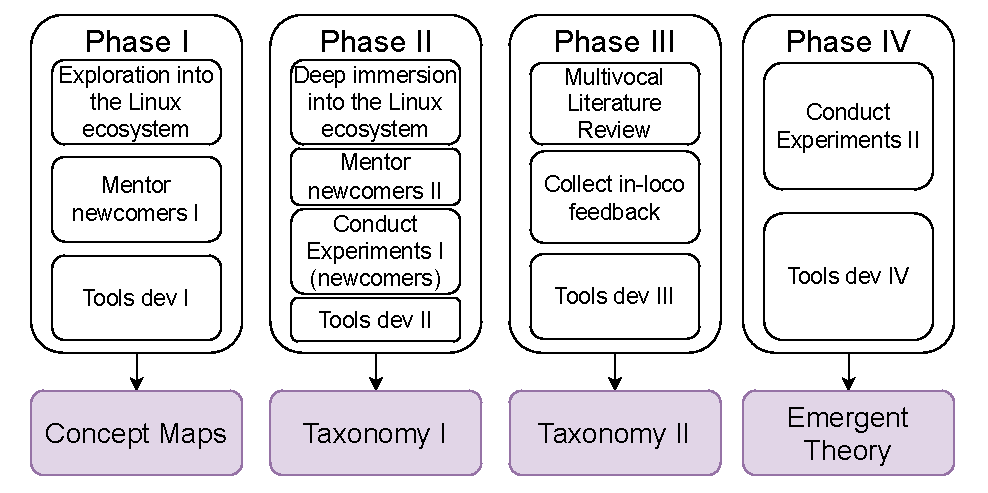
\includegraphics[width=0.8\textwidth]{images/phd-phases.pdf}
    \caption{Research work plan.\label{fig:research-work-plan}}
\end{figure}

Figure \ref{fig:research-work-plan} is a diagram that summarizes the four phases. In this figure, each phase also describes the core work it represents (blue boxes at the middle of the figure), along with the iteration of the theoretical framework produced by the phase (magenta boxes at the bottom).

\subsection{Execution Schedule}

Given the tasks of each phase, Table \ref{tab:work-plan} describes the five-year (60 months) schedule for this proposed doctoral research. \textbf{P0} refers to Phase 0 regarding the courses the doctoral student has to attend as part of his post-graduation program. For better visualization, activities in italics and underlined pertain to development tasks. Also, the cyan color represents the terms when the doctoral student plans to do a \textit{Research Internship Abroad} (RIA) to Spain at the \textit{Rey Juan Carlos University} (URJC), which is already agreed with the RIA advisor.

\begin{table}[htb]
\small
\centering
\caption{60 months schedule for the proposed doctoral research.}
\label{tab:work-plan}
\begin{tabular}{|c|c|c|c|c|c|c|c|c|c|c|}
\hline
\rowcolor{lightgray}
Activity &
\multicolumn{1}{c|}{\begin{tabular}[c]{@{}c@{}}24.1\end{tabular}} &
\multicolumn{1}{c|}{\begin{tabular}[c]{@{}c@{}}24.2\end{tabular}} &
\multicolumn{1}{c|}{\begin{tabular}[c]{@{}c@{}}25.1\end{tabular}} &
\multicolumn{1}{c|}{\begin{tabular}[c]{@{}c@{}}25.2\end{tabular}} &
\multicolumn{1}{c|}{\begin{tabular}[c]{@{}c@{}}26.1\end{tabular}} &
\multicolumn{1}{c|}{\begin{tabular}[c]{@{}c@{}}\cellcolor[HTML]{CCCCFF}26.2\end{tabular}} &
\multicolumn{1}{c|}{\begin{tabular}[c]{@{}c@{}}\cellcolor[HTML]{CCCCFF}27.1\end{tabular}} &
\multicolumn{1}{c|}{\begin{tabular}[c]{@{}c@{}}27.2\end{tabular}} &
\multicolumn{1}{c|}{\begin{tabular}[c]{@{}c@{}}28.1\end{tabular}} &
\multicolumn{1}{c|}{\begin{tabular}[c]{@{}c@{}}28.2\end{tabular}} \\ \hline
\cellcolor[gray]{0.8}\textbf{P0.0} & X & X & X & X & & \cellcolor[HTML]{CCCCFF}  & \cellcolor[HTML]{CCCCFF} &   &   & \\ \hline
\cellcolor[gray]{0.8}\textbf{P1.1} & X & X & X &   & & \cellcolor[HTML]{CCCCFF}  & \cellcolor[HTML]{CCCCFF} &   &   &   \\ \hline
\cellcolor[gray]{0.8}\textbf{P1.2} & X &   &   &   & & \cellcolor[HTML]{CCCCFF}  & \cellcolor[HTML]{CCCCFF} &   &   &   \\ \hline
\cellcolor[gray]{0.8}\underline{\textit{\textbf{P1.3}}} & X & X & & & & \cellcolor[HTML]{CCCCFF}  & \cellcolor[HTML]{CCCCFF} &   &   &   \\ \hline
\cellcolor[gray]{0.8}\textbf{P2.1} &   &   & X & X & X & \cellcolor[HTML]{CCCCFF}  & \cellcolor[HTML]{CCCCFF}  &   &   &   \\ \hline
\cellcolor[gray]{0.8}\textbf{P2.2} &   &   & X &   &   & \cellcolor[HTML]{CCCCFF}  & \cellcolor[HTML]{CCCCFF}  &   &   &   \\ \hline
\cellcolor[gray]{0.8}\textbf{P2.3} &   &   & X &   &   & \cellcolor[HTML]{CCCCFF}  & \cellcolor[HTML]{CCCCFF}  &   &   &   \\ \hline
\cellcolor[gray]{0.8}\underline{\textit{\textbf{P2.4}}} &   &   & X & X & X & \cellcolor[HTML]{CCCCFF}  & \cellcolor[HTML]{CCCCFF} &   &   &   \\ \hline
\cellcolor[gray]{0.8}\textbf{P3.1} &   &   &   &   & X & \cellcolor[HTML]{CCCCFF}X & \cellcolor[HTML]{CCCCFF}X & X &   &   \\ \hline
\cellcolor[gray]{0.8}\textbf{P3.2} &   &   & X & X & X & \cellcolor[HTML]{CCCCFF}X & \cellcolor[HTML]{CCCCFF}X &   &   &   \\ \hline
\cellcolor[gray]{0.8}\underline{\textit{\textbf{P3.3}}} &   &   &   &   & & \cellcolor[HTML]{CCCCFF}X & \cellcolor[HTML]{CCCCFF}X & X &   &   \\ \hline
\cellcolor[gray]{0.8}\textbf{P4.1} &   &   &   &   &  & \cellcolor[HTML]{CCCCFF}  & \cellcolor[HTML]{CCCCFF} & X & X &   \\ \hline
\cellcolor[gray]{0.8}\underline{\textit{\textbf{P4.2}}} &   &   &   &   &  & \cellcolor[HTML]{CCCCFF}  & \cellcolor[HTML]{CCCCFF} & X & X & X \\ \hline
\end{tabular}
\normalsize
\end{table}
